\documentclass{article}
\usepackage[utf8]{inputenc}
\usepackage{graphicx}
\usepackage{amsmath}
\usepackage{amsfonts}
\usepackage{amssymb}
\usepackage{float}

\usepackage{listings}
\usepackage{hyperref}

\newcommand{\mail}[1]{{\href{mailto:#1}{#1}}}


\begin{document}
\title{RandomFruitDB}
\author{Tristan Henchoz, Arthur Morgan, Mattéo Bonvin
	\\ {\small\mail{tristan.henchoz@unifr.ch, arthur.morgan@unifr.ch, matteo.bonvin@unifr.ch}}}
\date{\today}

\maketitle
\tableofcontents
\pagebreak


\section{Problem Statement}
RandomFruitDB is a distributed database system using the Elixir programming language. A distributed database is a database that is distributed across multiple computers, usually connected through a network. In a distributed database system, data is stored and managed in multiple physical locations, each with its own database management system (DBMS). The goal of a distributed database is to provide users with the ability to access and modify data from anywhere while providing fault tolerance and data availability.
\\\\
Distributed databases differ from traditional centralized databases because they are designed to handle large amounts of data. Data and high-level consensus support distribution processes and distribution decision-making processes. They also typically provide features such as data partitioning and replication that allow data to be stored and accessed in multiple locations to improve performance and reliability.
\\\\
This type of database faces a number of challenges. Firstly, they are more complex to set up, maintain, and troubleshoot than traditional single-server databases. In addition, they can potentially suffer from performance problems due to their complexity. Another major challenge they face is data consistency. They must ensure that data updates from one computer are correctly applied to all other computers. Finally, scalability is an issue for a distributed database because adding new computers adds complexity and can result in performance losses.
\\\\
With RandomFruitDB, we try to solve these problems with the Chord algorithm. Peer-to-peer file sharing systems use the Distributed Hash Table (DHT), which is a Chord algorithm. Even though the network is constantly being joined and left, this allows the network to efficiently access and receive information from other networks. Each node has a unique ID. A large number is usually chosen from a random distribution. Each ID is higher than the previous one and lower than the next in a logical hierarchy. This space is called the code space. A list of other nodes in the network is maintained in a table called a fingerprint. A hash table is used to route data requests in the network.
\\\\
When a person wants to join the network, they send a request to another person to find a successor. The location of the new node is reflected in its fingerprints. To receive data from the network, a node checks the data store to see if it is available. The request is sent to the next highest queue ID. If the data is not in the network, this process is repeated. The ability to efficiently manage nodes entering and leaving the network is an important feature of the Chord Algorithm. The proxy takes and updates the finger table when a node is offline. The finger table is updated when a new node joins the network. The Chord is an efficient way to access and get information from each other. It is used in many distribution systems. 
\cite{ref1}

\begin{figure}[h]
\centering
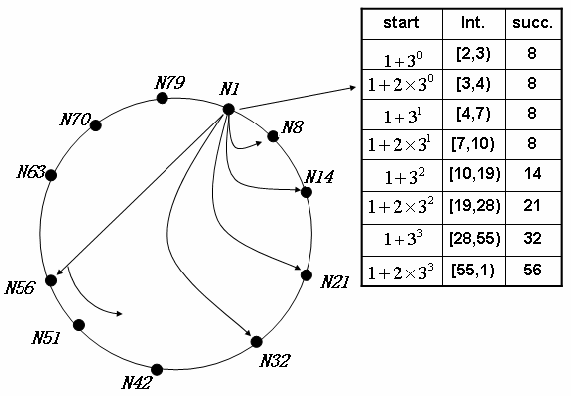
\includegraphics[width=\textwidth]{img/ChordAlgorithm}
\caption{A Bidirectional Chord System Based on Base-k Finger Table}
\label{figure 1}
\end{figure}

\pagebreak

\section{State-of-the-art}

Distributed databases are designed to store and manage large amounts of data across multiple servers, typically in a cluster or a grid. They allow for high availability, scalability, and fault tolerance by distributing the data and processing workload across multiple nodes.
There are several different types of distributed databases, including:
\begin{enumerate}
\item NoSQL distributed databases: These databases are designed to handle large amounts of data that may be structured, semi-structured, or unstructured. They often use non-relational data models, such as key-value stores, document stores, and column-family stores. 
\cite{ref2}

Examples include MongoDB, Cassandra, and HBase.
\item Relational distributed databases: These are traditional database management systems (DBMS) that have been extended to support distributed storage and processing. Examples include MySQL Cluster and Oracle RAC.
\item NewSQL distributed databases: These are a newer class of databases that combine the scalability and high performance of NoSQL databases with the Atomicity, Consistency, Isolation and Durability (ACID) properties and SQL interface of traditional relational databases . Examples include CockroachDB and TiDB. 
\cite{ref3}

\end{enumerate}
Another way to classify distributed databases is by the way they store and replicate data: 
\cite{ref4}

\begin{enumerate}
\item Shared-nothing architecture: In this type of distributed database, each node operates independently and has its own local storage. Data is partitioned and distributed among the nodes, and there is no central coordination or shared resources. This allows for high scalability and fault tolerance but can make it more difficult to maintain consistency and integrity. Examples include Cassandra and HBase.
\item Shared-nothing architecture with distributed consensus: In this type of distributed database, multiple nodes operate independently and have their own local storage, but they use a distributed consensus protocol to ensure data integrity and consistency. This allows for high scalability and fault tolerance, as well as strong consistency guarantees. Examples include Google Cloud Spanner and CockroachDB.
\item Shared-disk architecture: In this type of distributed database, multiple nodes share access to a common storage system, such as a SAN (storage area network). Data is partitioned and distributed among the nodes, but each node can access the data stored on the shared disk. This allows for easier maintenance of consistency and integrity but can be less scalable and less tolerant to failures. Examples include Oracle RAC and Sybase IQ.
\end{enumerate}
Our system would therefore be part of the NoSQL distributed databases with a Shared-nothing architecture


\section{Presentation of the solution}
Our distributed database is implemented by a simplified chord node. We successfully create a ring and nodes within it, as well as communication between the nodes on the ring. The creation of the nodes and ring, as well as sending requests to the node is done by a dispatcher.
\\\\
When putting a file in our database, the dispatcher will select a node in the ring and assign the file to it. When looking for a file in our database, the dispatcher will select a node, but if the node doesn't have the file it will ask the following node in the ring if it has the file. When a node with the file has been found it will answer to the dispatcher directly. We also aimed to have a hash file that would have helped distribute the files more evenly and find them more efficiently. Having a hash table would also have allowed for better integrity, as we could have correctly updated files and avoid conflicts.
\\\\
We also wanted to use MongoDB as a backend database to properly store each node's data for simplificication.
\\\\
On the frontend we aimed to have a web app interface that we can use to store and find files.
\\\\

\section{Validation \& evaluation of the solution}

Our solution bypasses a number of rules to create a simplificication of a real chord system. One of these simplificications is the order of the node and the file classification, as it is done randomly to avoid dealing with hash calculation. The solution is therefore simple, but it keeps its academic purpose.
\\\\
Another simplificication we made is the creation and the use of a "dispatcher", which manages adding new nodes in the ring and manages data communication within the ring. This system is purely here for simplicity, and doesn't have any academic interest.
\\\\
Our simplified node will connect directly to the dispatcher when created, and the latter will assign to them a position in the ring. The node will then take care of notifying the other nodes of its presence. Our ring could in part refresh and correct its state (next node) on its own, but the feature wasn't developed enough to be able to avoid some unexpected errors.
\begin{figure}[H]
  \centering
  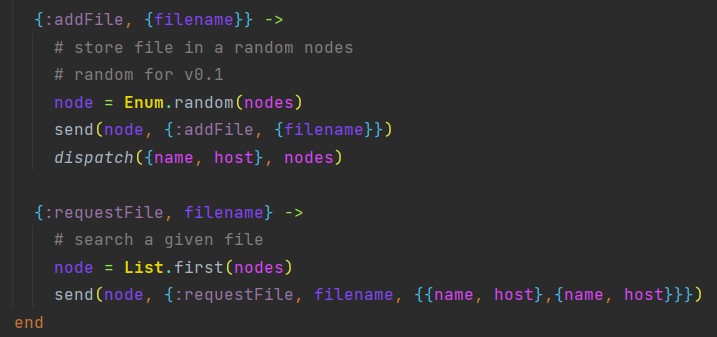
\includegraphics[width=\textwidth]{img/dispatch.png}
  \caption{A part of the dispatcher.}
  \label{figure 2 :}
\end{figure}
The main part of our system is the possibility to retreive data. Storing a file is simple, as the dispatcher randomly selects a node to store it (to avoid the use of a hash table). To retreive data, the dispatcher will randomly ask a node. The node will either answer with the file or it will ask the next node for it. A condition is put to avoid circular search, and when a file is found it is send directly to the dispatcher and does not circle back.
\\\\
For the frontend part of the project, we developed a simple HTML page of the database with minimal styling using JavaScript code, including colours and a hover effect for the buttons. 
The page has three parts: the first one allows to search the database and should show the results of the search. The second is for adding a document. The last one is the list of documents added from this computer which appears as a list :

\begin{figure}[H]
  \centering
  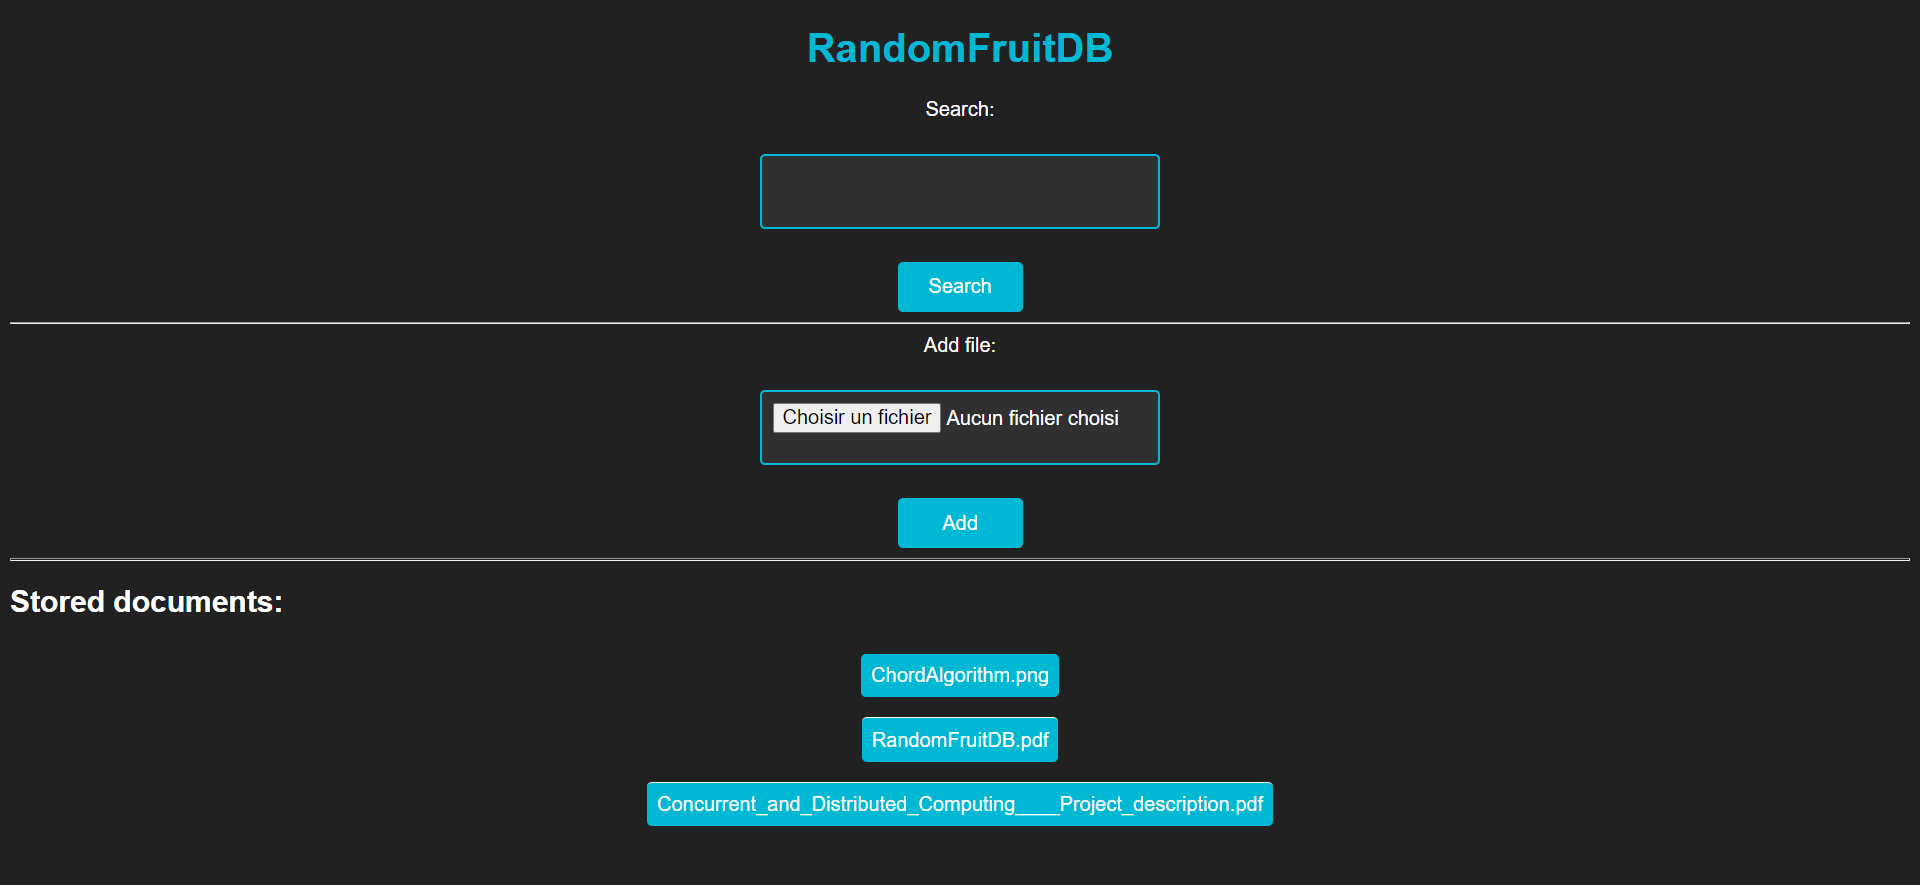
\includegraphics[width=\textwidth]{img/html.png}
  \caption{The HTML frontend.}
  \label{figure 3 :}
\end{figure}


\section{Discussion of the results}
Our solution is currently not working, mainly because of the treatment of files using Elixir. We did manage to implement the ring, it can store data (currently file names only) on multi node, and retreive this data without having to connect to the node on which the information is located.
\\\\
The part we struggled with the most is the communication between the frontend and the backend. The frontend sends requests to the backend but we couldn't get implement a request handler that would properly work and display the results in the browser.
\\\\
Our solution doesn't create a finished and out-of-the box system. The main issue is the lack of backend-frontend communication. Because we weren't able to achieve our base objectives, there is still a lot of room to improve and further develop.
\\\\
We did manage to achieve one of our main goals, which was to implement a simplified chord system. Without the use of a hash table, the ring doesn't maintain a stable state and files can't actually be used, but even with these limitation, the academic purpose of understading chord systems, it's limitations and difficulties, was still achieved.




\pagebreak

\begin{thebibliography}{9}
\bibitem{ref1}
Minghui Ji, "Hierarchical Bidirectional Chord," 2010 International Conference on Educational and Information Technology, 2010, pp. V3-486-V3-489, doi: 10.1109/ICEIT.2010.5607543.
\bibitem{ref2}
Y. Zhou, Q. Chen, B. Shan, F. Jiang and Y. Pang, "A Distributed Storage Strategy For Trajectory Data Based On Nosql Database," IGARSS 2019 - 2019 IEEE International Geoscience and Remote Sensing Symposium, 2019, pp. 3487-3490, doi: 10.1109/IGARSS.2019.8900482.
\bibitem{ref3}
K. Kaur and M. Sachdeva, "Performance evaluation of NewSQL databases," 2017 International Conference on Inventive Systems and Control (ICISC), 2017, pp. 1-5, doi: 10.1109/ICISC.2017.8068585.
\bibitem{ref4}
Simic, Sofija, "Shared Nothing Architecture Explained (Diagram, Pros \& Cons)". Knowledge Base by phoenixNAP, 2 septembre 2021. https://phoenixnap.com/kb/shared-nothing-architecture.
\bibitem{ref5}
Image Reference : H. Yan, Y. Jiang and X. Zhou, "A Bidirectional Chord System Based on Base-k Finger Table," 2008 International Symposium on Computer Science and Computational Technology, 2008, pp. 384-388, doi: 10.1109/ISCSCT.2008.55.
\end{thebibliography}

\pagebreak

\appendix

 \section{Readme}
 To make a 3 nodes circle:
 \begin{enumerate}
  \item Create bridge network
  \item[] \texttt{docker network create elixir-net docker network inspect elixir-net }
  \item Start Docker containers in network
  \begin{itemize}
   \item First terminal
   \item[] \texttt{docker run -rm -it -name elixir1 -h host1 -net elixir-net elixir /bin/bash }
   \item Second terminal
   \item[] \texttt{docker run -rm -it -name elixir1 -h host1 -net elixir-net elixir /bin/bash}
   \item Third terminal
   \item[] \texttt{docker run -rm -it -name elixir3 -h host3 -net elixir-net elixir /bin/bash}
   \item Fourth terminal
   \item[] \texttt{docker run -rm -it -name elixir4 -h host4 -net elixir-net elixir /bin/bash}
  \end{itemize}
  \item Run elixir
  \begin{itemize}
   \item First terminal
   \item[] \texttt{iex --sname foo --cookie secret}
   \item Second terminal
   \item[] \texttt{iex --sname bar --cookie secret}
   \item Third terminal
   \item[] \texttt{iex --sname bof --cookie secret}
   \item Fourth terminal
   \item[] \texttt{iex --sname dis --cookie secret}
  \end{itemize}
  \item Run Program
  \begin{itemize}
   \item First terminal
   \item[] \texttt{Node.ping(:bar@host2)}
   \item Second terminal
   \item[] \texttt{Node.ping(:bar@host2)}
   \item Third terminal
   \item[] \texttt{Node.ping(:bar@host2)}
   \item Fourth terminal
   \item[] \texttt{Node.ping(:bar@host2)}
  \end{itemize}
  \begin{enumerate}
   \item Copy file (assuming the file are in the local directory)
   \item[] \texttt{docker cp communication.ex elixir1:communication.ex}
   \item[] \texttt{docker cp communication.ex elixir2:communication.ex}
   \item[] \texttt{docker cp communication.ex elixir3:communication.ex}
   \item[] \texttt{docker cp nodes.ex elixir1:nodes.ex}
   \item[] \texttt{docker cp nodes.ex elixir2:nodes.ex}
   \item[] \texttt{docker cp nodes.ex elixir3:nodes.ex}
   \item[] \texttt{docker cp dispatcher.ex elixir4:dispatcher.ex}
   \item Compile DB program
   \begin{itemize}
   \item First, second and third terminal
   \item[] \texttt{c("communication.ex")}
   \item[] \texttt{c("nodes.ex")}
   \item Fourth terminal
   \item[] \texttt{c("dispatcher.ex")}
   \end{itemize}

   \item Run DB Program
  \begin{itemize}
   \item Fourth terminal (has to be done first)
   \item[] \texttt{Dispatcher.initiate(:dis@host4)}
   \item First terminal
   \item[] \texttt{Process.register(Nodee.node\_init({:n1, :foo@host1}, {:dispatcher, :dis@host4}), :n1)}
   \item Second terminal
   \item[] \texttt{Process.register(Nodee.node\_init({:n2, :bar@host2}, {:dispatcher, :dis@host4}), :n2)}
   \item Third terminal
   \item[] \texttt{Process.register(Nodee.node\_init({:n3, :bof@host3}, {:dispatcher, :dis@host4}), :n3)}
  \end{itemize}
  \item Usage in fourth terminal
  \item[] Add files:
  \item[] \texttt{Dispatcher.addFile("SampleFile1”)}
  \item[] \texttt{Dispatcher.addFile("SampleFile2”)}
  \item[] Find files:
  \item[] \texttt{Dispatcher.lookFile("SampleFile1”)}
  \end{enumerate}
  \item Clean up
  \item[] \texttt{docket network rm elixir-net}
 \end{enumerate}

\end{document}

